\documentclass[a4paper, 12pt]{article}
\usepackage[a4paper,top=1.5cm, bottom=1.5cm, left=1cm, right=1cm]{geometry}

% Работа с русским языком
\usepackage[utf8]{inputenc}
\usepackage{mathtext}                % русские буквы в формулах
\usepackage[english, russian]{babel} % локализация и переносы

\usepackage{graphicx}   % Вставка изображений
\usepackage{float}      % "Плавающие" изображения3
\usepackage{wrapfig}    % Обтекание фигур (таблиц, картинок и прочего)
\graphicspath{ {./images/} }

\usepackage{tabularx}
\usepackage{multirow}
\usepackage{amsmath}
\usepackage{amsfonts}
\usepackage{indentfirst}
\usepackage{longtable}
\graphicspath{{pictures/}}
\usepackage{natbib}

%%% Колонтитулы
\usepackage{titleps}
\newpagestyle{main}{
	\setheadrule{0.4pt}
	\sethead{Измерение осмотического давления}{}{}
	\setfootrule{0.4pt}                       
	\setfoot{ФРКТ МФТИ, 2023}{}{\thepage} 
}
\pagestyle{main}  

\begin{document}
    \begin{titlepage}
	\begin{center}
            {\large МОСКОВСКИЙ ФИЗИКО-ТЕХНИЧЕСКИЙ ИНСТИТУТ (НАЦИОНАЛЬНЫЙ       ИССЛЕДОВАТЕЛЬСКИЙ УНИВЕРСИТЕТ)}
	\end{center}
 
	\begin{center}
		{\large Физтех-школа радиотехники и компьютерных технологий}
	\end{center}
	
	\vspace{8cm}
	{\LARGE
		\begin{center}
                {\bf Вопрос по выбору для экзамена по термодинамике}\\
                Измерение осмотического давления
		\end{center}
	}
	\vspace{5cm}
	\begin{flushright}
		{\Large Автор:\\ Тихонов Дмитрий Романович, \\
			\vspace{0.2cm}
			студент группы Б01-206}
	\end{flushright}
	\vspace{5cm}
	\begin{center}
		\Large Долгопрудный, 2023
	\end{center}
    \end{titlepage}

    \section{Введение}

    \noindent \textbf{Цель работы:}  
    \begin{enumerate}
        \item измерение осмотического давления при разной концентрации жёлтой кровяной соли;
        \item проверка закона Вант-Гоффа.
    \end{enumerate}

    \noindent \textbf{В работе используются:} осмометр; секундомер; пипетка; мерный стаканчик; химический стакан.
    
    \section{Теоретические сведения}

    \noindent В работе изучаются свойства \textit{полупроницаемых перегородок}, т. е. таких перегородок, которые пропускают молекулы растворителя, но не пропускают молекулы растворённых в ней соединений. Прохождение растворителя через полупроницаемую перегородку называется \textit{осмосом}. \\
    
    \noindent Так, многие перепонки и мембраны животного и растительного происхождения свободно пропускают молекулы воды, но не пропускают молекулы растворенных в ней соединений, обладающих большей молекулярной массой. \\
    
    \noindent Рассмотрим сосуд (рис. \ref{th:osm}), разделённый на две части полупроницаемой перегородкой, по одну сторону которой находится вода, а по другую - водный раствор вещества, молекулы которого не могут проходить сквозь перегородку. Наполним обе части сосуда до одинакового уровня. 

    \begin{figure}[H]
        \centering
        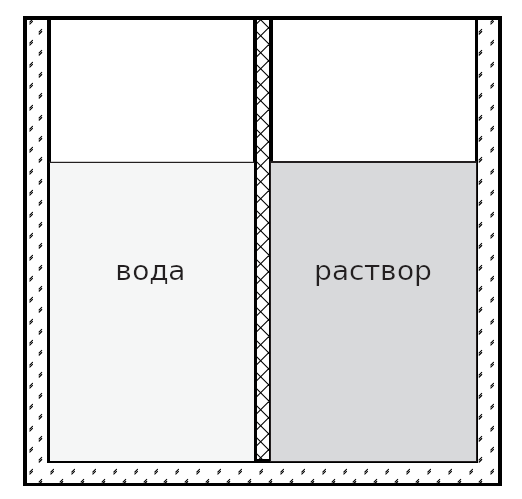
\includegraphics[scale = 0.5]{images/scheme_theory.png}
        \caption{Сосуд, разделенный на две части перегородкой}
        \label{th:osm}
    \end{figure}
    
    \noindent Опыт показывает, что вода начинает переходить в ту часть сосуда, где содержится раствор. Этот переход продолжается до тех пор, пока между водой и раствором не установится некоторая разность уровней (рис. \ref{th:osm_eq}), а следовательно, и разность давлений, которая носит название \textit{осмотического давления раствора}. 

    \begin{figure}[H]
        \centering
        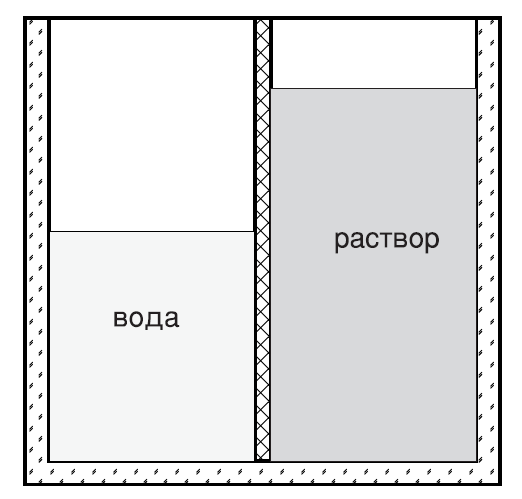
\includegraphics[scale = 0.5]{images/scheme_theory_eq.png}
        \caption{Положение уровней жидкостей в момент окончания перехода}
        \label{th:osm_eq}
    \end{figure}
    
    \noindent Осмотическое давление подчиняется закону Вант-Гоффа:

    \begin{equation}
        \label{osm}
        P_\text{осм} = nkT,
    \end{equation}

    \noindent где $n$ - число молекул растворенного вещества в единице объема, $k$ - постоянная Больцмана, $T$ - абсолютная температура. Формула \ref{osm} позволяет по известной величине $P_\text{осм}$ определить концентрацию молекул растворенного вещества.
    
    \section{Методика измерений и используемое оборудование}

    \noindent Приборы, служащие для измерения осмотического давления, называют \textit{осмометрами}. Прохождение растворителя через полупроницаемые перегородки происходит медленно, так что равновесие раствора и растворителя устанавливается не скоро. Для ускорения измерений над раствором создают избыточное давление воздуха. Если избыточное давление равно осмотическому, то переход растворителя через перегородку прекращается. Если же оно превышает осмотическое давление, то растворитель переходит через перегородку в обратном направлении. Таким образом, измерение осмотического давления сводится к измерению равновесного давления газа. Схема используемого в работе осмометра приведена на рис. \ref{installation}. 

    \begin{figure}[H]
        \centering
        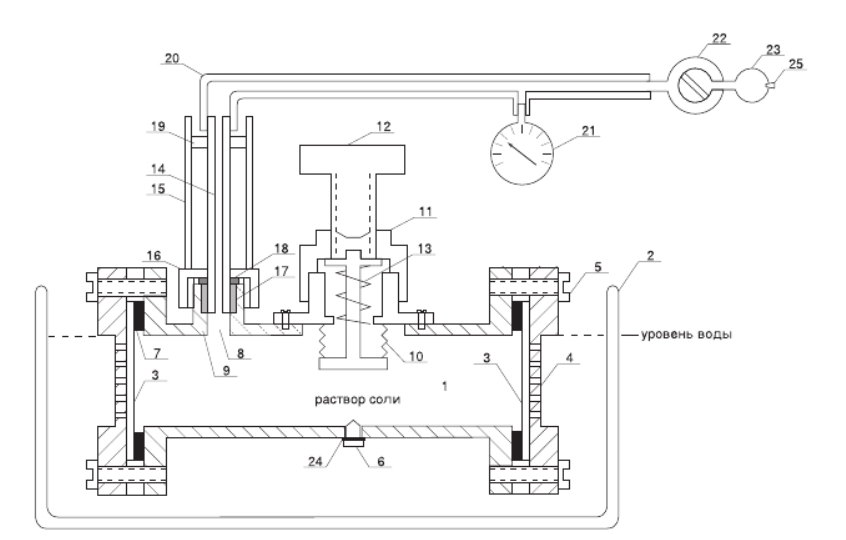
\includegraphics[scale = 0.5]{images/installation.png}
        \caption{Осмометр, используемый в данной работе}
        \label{installation}
    \end{figure}
    
    \noindent Раствор заливается в контейнер, который помещается в сосуд с растворителем. Контейнер представляет собой куб $1$, закрытый с четырёх сторон полупроницаемыми целлофановыми мембранами $3$ толщиной $0,2$ мм. Мембраны зажимаются между стенками куба $1$ и металлическими сетками $4$. Между мембранами и стенками куба вставлены резиновые уплотнения $7$. Защитные сетки $4$ предохраняют мембраны от раздувания наружу. Сосуд заполняется раствором через отверстие в дне куба, плотно закрываемое металлической гайкой $6$ с резиновой прокладкой $24$. Через крышку куба вставлен стеклянный капилляр $14$ (внутренний диаметр $0,5$ мм). В процессе осмоса объём раствора увеличивается, и уровень раствора движется по капилляру вверх. Скорость подъёма уменьшается при избыточном давлении воздуха на верхнем конце капилляра; оно создаётся с помощью резиновой груши $23$ со встроенным клапаном $25$ и фиксируется краном $22$. Давление измеряется манометром $21$. Кран $22$ позволяет сбросить избыточное давление. На крышке куба $1$ смонтировано устройство, состоящее из гофра $10$, накидной гайки $11$, винта $12$ и пружины $13$, позволяющее менять объём внутреннего пространства в кубе. Это бывает необходимо, если в процессе опыта мембраны вытягиваются и уровень раствора в капилляре понижается. При закручивании винта $12$ объём контейнера уменьшается и раствор вытесняется в капилляр. Таким образом, уровень раствора можно установить в капилляре на удобной для наблюдения высоте. \\
    
    \noindent Для определения $P_\text{осм}$ измеряют изменение скорости $v$ движения уровня раствора в капилляре в зависимости от давления воздуха $Р$ и строят график зависимости $v(P)$. Чем больше разность давления $P - P_\text{осм}$, тем больше скорость $v$ движения уровня в капилляре. При $P \approx P_\text{осм}$ эта скорость равна нулю. Поэтому измерения следует проводить либо при $P \gg P_\text{осм}$, либо при $Р \ll P_\text{осм}$. По графику легко определить значение Р, при котором $v = 0$, т. е. осмотическое давление $P_\text{осм}$.\\
    
    \noindent В работе измеряется осмотическое давление водного раствора жёлтой кровяной соли $K_4 Fe (CN)_6$, при нескольких значениях концентрации и проверяется справедливость закона Вант-Гоффа. Молекулы жёлтой кровяной соли при растворении диссоциируют: $K_4 Fe (CN)_6 \rightarrow 4K^{+} +[Fe (CN)_6]^{4-}$. Ионы $К^+$ свободно проникают через нашу перегородку и не создают осмотического давления.

    \section{Результаты измерений и обработка данных}

    \noindent В работе для каждой концентрации раствора сначала проводились измерения при давлениях $Р \gg P_\text{осм}$. Начальное давление устанавливалось $Р = 200$ делений, затем оно понижалось до тех пор, пока давление достаточно больше осмотического, чтобы время эксперимента не было слишком большим. \\
    
    \noindent После этого измерения проводились при давлениях $P \ll P_\text{осм}$, при этом можно было наблюдать повышение уровня жидкости в капилляре. Прямой осмос удалось наблюдать только при давлении $Р = 0$ делений. \\
    
    \noindent Предел измерений манометра, используемого в работе равен $P_\text{пр} = 400 \text{ дел} = 1 = 98066 \text{ Па}$. Цена деления равна $P_\text{ц.д.} = 1 \text{ дел} = 245 \text{ Па}$. Инструментальная погрешность измерения $\sigma_P = 1 \text{ дел}$. \\

    \noindent Приведём результаты измеренных значений для разных концентраций раствора.

    \subsection{Измерение осмотического давления для раствора концентрацией 0,3\%}
        \begin{table}[H]
            \centering
            \begin{tabular}{|c|ccccc|}
            \hline
            $P$, дел. & \multicolumn{1}{c|}{$t$, с} & \multicolumn{1}{c|}{$l$, см} & \multicolumn{1}{c|}{$u$, $10^{-4} \cdot$м/с} & \multicolumn{1}{c|}{$\overline{u}$, $10^{-4} \cdot$м/с} & $\sigma_{\overline{u}}$, $10^{-4} \cdot$м/с \\ \hline
            \multirow{5}{*}{200} & \multicolumn{1}{c|}{27,48} & \multicolumn{1}{c|}{\multirow{5}{*}{2}} & \multicolumn{1}{c|}{7,28} & \multicolumn{1}{c|}{\multirow{5}{*}{7,38}} & \multirow{5}{*}{0,10} \\ \cline{2-2} \cline{4-4}
             & \multicolumn{1}{c|}{27,51} & \multicolumn{1}{c|}{} & \multicolumn{1}{c|}{7,27} & \multicolumn{1}{c|}{} &  \\ \cline{2-2} \cline{4-4}
             & \multicolumn{1}{c|}{26,81} & \multicolumn{1}{c|}{} & \multicolumn{1}{c|}{7,46} & \multicolumn{1}{c|}{} &  \\ \cline{2-2} \cline{4-4}
             & \multicolumn{1}{c|}{26,44} & \multicolumn{1}{c|}{} & \multicolumn{1}{c|}{7,56} & \multicolumn{1}{c|}{} &  \\ \cline{2-2} \cline{4-4}
             & \multicolumn{1}{c|}{27,27} & \multicolumn{1}{c|}{} & \multicolumn{1}{c|}{7,33} & \multicolumn{1}{c|}{} &  \\ \hline
            \multirow{5}{*}{180} & \multicolumn{1}{c|}{30,46} & \multicolumn{1}{c|}{\multirow{5}{*}{2}} & \multicolumn{1}{c|}{6,57} & \multicolumn{1}{c|}{\multirow{5}{*}{6,50}} & \multirow{5}{*}{0,06} \\ \cline{2-2} \cline{4-4}
             & \multicolumn{1}{c|}{30,32} & \multicolumn{1}{c|}{} & \multicolumn{1}{c|}{6,60} & \multicolumn{1}{c|}{} &  \\ \cline{2-2} \cline{4-4}
             & \multicolumn{1}{c|}{30,76} & \multicolumn{1}{c|}{} & \multicolumn{1}{c|}{6,50} & \multicolumn{1}{c|}{} &  \\ \cline{2-2} \cline{4-4}
             & \multicolumn{1}{c|}{31,20} & \multicolumn{1}{c|}{} & \multicolumn{1}{c|}{6,41} & \multicolumn{1}{c|}{} &  \\ \cline{2-2} \cline{4-4}
             & \multicolumn{1}{c|}{31,07} & \multicolumn{1}{c|}{} & \multicolumn{1}{c|}{6,44} & \multicolumn{1}{c|}{} &  \\ \hline
            \multirow{5}{*}{160} & \multicolumn{1}{c|}{33,68} & \multicolumn{1}{c|}{\multirow{5}{*}{2}} & \multicolumn{1}{c|}{5,94} & \multicolumn{1}{c|}{\multirow{5}{*}{5,77}} & \multirow{5}{*}{0,17} \\ \cline{2-2} \cline{4-4}
             & \multicolumn{1}{c|}{33,14} & \multicolumn{1}{c|}{} & \multicolumn{1}{c|}{6,04} & \multicolumn{1}{c|}{} &  \\ \cline{2-2} \cline{4-4}
             & \multicolumn{1}{c|}{36,10} & \multicolumn{1}{c|}{} & \multicolumn{1}{c|}{5,54} & \multicolumn{1}{c|}{} &  \\ \cline{2-2} \cline{4-4}
             & \multicolumn{1}{c|}{35,30} & \multicolumn{1}{c|}{} & \multicolumn{1}{c|}{5,67} & \multicolumn{1}{c|}{} &  \\ \cline{2-2} \cline{4-4}
             & \multicolumn{1}{c|}{35,30} & \multicolumn{1}{c|}{} & \multicolumn{1}{c|}{5,67} & \multicolumn{1}{c|}{} &  \\ \hline
            \multirow{5}{*}{120} & \multicolumn{1}{c|}{45,94} & \multicolumn{1}{c|}{\multirow{5}{*}{2}} & \multicolumn{1}{c|}{4,35} & \multicolumn{1}{c|}{\multirow{5}{*}{4,30}} & \multirow{5}{*}{0,09} \\ \cline{2-2} \cline{4-4}
             & \multicolumn{1}{c|}{44,85} & \multicolumn{1}{c|}{} & \multicolumn{1}{c|}{4,46} & \multicolumn{1}{c|}{} &  \\ \cline{2-2} \cline{4-4}
             & \multicolumn{1}{c|}{46,79} & \multicolumn{1}{c|}{} & \multicolumn{1}{c|}{4,27} & \multicolumn{1}{c|}{} &  \\ \cline{2-2} \cline{4-4}
             & \multicolumn{1}{c|}{47,41} & \multicolumn{1}{c|}{} & \multicolumn{1}{c|}{4,22} & \multicolumn{1}{c|}{} &  \\ \cline{2-2} \cline{4-4}
             & \multicolumn{1}{c|}{47,76} & \multicolumn{1}{c|}{} & \multicolumn{1}{c|}{4,19} & \multicolumn{1}{c|}{} &  \\ \hline
            \multirow{5}{*}{80} & \multicolumn{1}{c|}{69,80} & \multicolumn{1}{c|}{\multirow{5}{*}{2}} & \multicolumn{1}{c|}{2,87} & \multicolumn{1}{c|}{\multirow{5}{*}{2,81}} & \multirow{5}{*}{0,06} \\ \cline{2-2} \cline{4-4}
             & \multicolumn{1}{c|}{69,81} & \multicolumn{1}{c|}{} & \multicolumn{1}{c|}{2,86} & \multicolumn{1}{c|}{} &  \\ \cline{2-2} \cline{4-4}
             & \multicolumn{1}{c|}{70,35} & \multicolumn{1}{c|}{} & \multicolumn{1}{c|}{2,84} & \multicolumn{1}{c|}{} &  \\ \cline{2-2} \cline{4-4}
             & \multicolumn{1}{c|}{72,71} & \multicolumn{1}{c|}{} & \multicolumn{1}{c|}{2,75} & \multicolumn{1}{c|}{} &  \\ \cline{2-2} \cline{4-4}
             & \multicolumn{1}{c|}{74,01} & \multicolumn{1}{c|}{} & \multicolumn{1}{c|}{2,70} & \multicolumn{1}{c|}{} &  \\ \hline
            40 & \multicolumn{5}{c|}{столб медленно опускается} \\ \hline
            20 & \multicolumn{5}{c|}{столб медленно понижается} \\ \hline
            10 & \multicolumn{5}{c|}{столб медленно поднимается} \\ \hline
            \multirow{5}{*}{0} & \multicolumn{1}{c|}{87,07} & \multicolumn{1}{c|}{\multirow{5}{*}{0,1}} & \multicolumn{1}{c|}{0,11} & \multicolumn{1}{c|}{\multirow{5}{*}{-0,11}} & \multirow{5}{*}{0,01} \\ \cline{2-2} \cline{4-4}
             & \multicolumn{1}{c|}{85,28} & \multicolumn{1}{c|}{} & \multicolumn{1}{c|}{0,12} & \multicolumn{1}{c|}{} &  \\ \cline{2-2} \cline{4-4}
             & \multicolumn{1}{c|}{87,94} & \multicolumn{1}{c|}{} & \multicolumn{1}{c|}{0,11} & \multicolumn{1}{c|}{} &  \\ \cline{2-2} \cline{4-4}
             & \multicolumn{1}{c|}{89,98} & \multicolumn{1}{c|}{} & \multicolumn{1}{c|}{0,11} & \multicolumn{1}{c|}{} &  \\ \cline{2-2} \cline{4-4}
             & \multicolumn{1}{c|}{86,23} & \multicolumn{1}{c|}{} & \multicolumn{1}{c|}{0,12} & \multicolumn{1}{c|}{} &  \\ \hline
            \end{tabular}
            \caption{Результаты измерений для первой концентрации раствора}
            \label{table:3per}
        \end{table}

        \noindent Построим график зависимости (рис. \ref{graph:3per}) давления воздуха $P$ от изменения скорости $v$ движения уровня раствора в капилляре для раствора с концентрацией $0,3 \%$. \\

        \noindent Аппроксимацию прямой произведем методом наименьших квадратов в компьютерной программе \textit{Origin Pro 2023}, в которой определим координату пересечения графика $P(v)$ с осью ординат. Получим:

        $$
        \boxed{P_\text{осм} = 6,0 \pm 2,3 \text{ дел} = 1470 \pm 564 \text{ Па}}
        $$

        \begin{figure}[H]
            \centering
            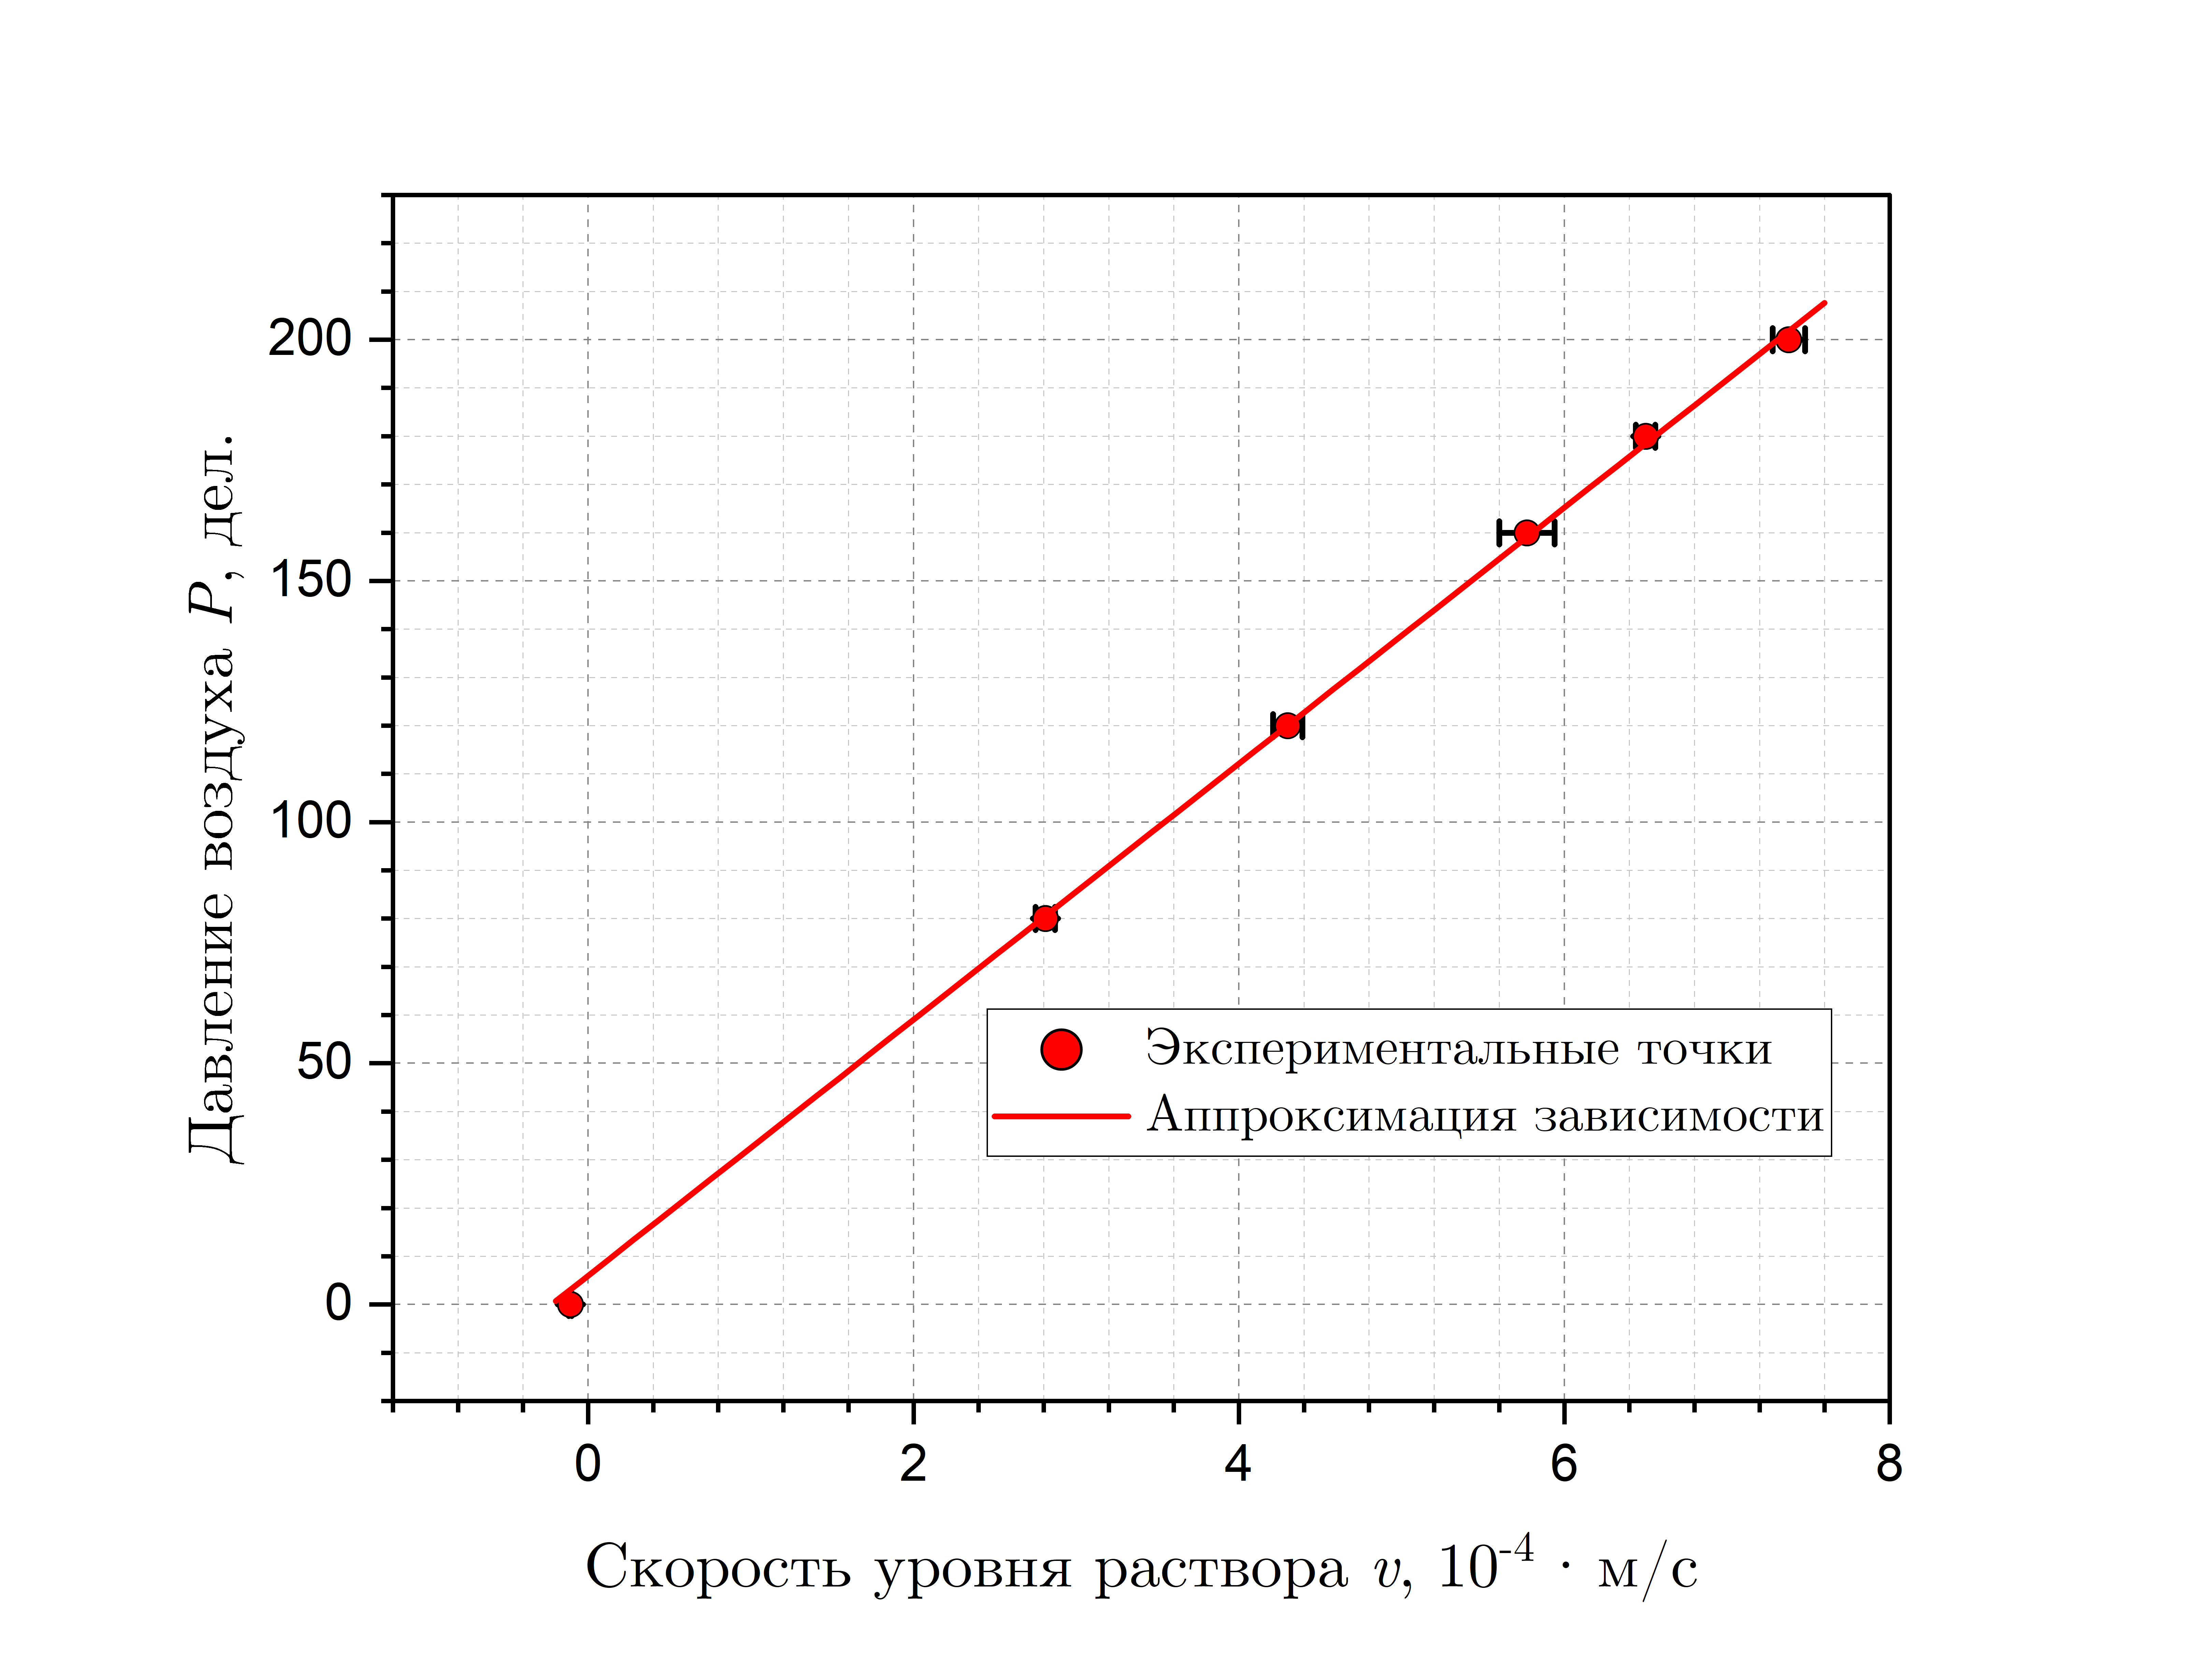
\includegraphics[width = 14 cm]{images/graph_3per.png}
            \caption{График зависимости $P(v)$ для первой концентрации раствора}
            \label{graph:3per}
        \end{figure}

        \subsection{Измерение осмотического давления для раствора концентрацией 0,15\%}
        
        \begin{table}[H]
            \centering
            \begin{tabular}{|c|ccccc|}
            \hline
            $P$, дел. & \multicolumn{1}{c|}{$t$, с} & \multicolumn{1}{c|}{$l$, см} & \multicolumn{1}{c|}{$u$, $10^{-4} \cdot$м/с} & \multicolumn{1}{c|}{$\overline{u}$, $10^{-4} \cdot$м/с} & $\sigma_{\overline{u}}$, $10^{-4} \cdot$м/с \\ \hline
            \multirow{5}{*}{200} & \multicolumn{1}{c|}{23,69} & \multicolumn{1}{c|}{\multirow{5}{*}{2}} & \multicolumn{1}{c|}{8,44} & \multicolumn{1}{c|}{\multirow{5}{*}{7,85}} & \multirow{5}{*}{0,24} \\ \cline{2-2} \cline{4-4}
             & \multicolumn{1}{c|}{25,47} & \multicolumn{1}{c|}{} & \multicolumn{1}{c|}{7,85} & \multicolumn{1}{c|}{} &  \\ \cline{2-2} \cline{4-4}
             & \multicolumn{1}{c|}{25,60} & \multicolumn{1}{c|}{} & \multicolumn{1}{c|}{7,81} & \multicolumn{1}{c|}{} &  \\ \cline{2-2} \cline{4-4}
             & \multicolumn{1}{c|}{26,34} & \multicolumn{1}{c|}{} & \multicolumn{1}{c|}{7,59} & \multicolumn{1}{c|}{} &  \\ \cline{2-2} \cline{4-4}
             & \multicolumn{1}{c|}{26,50} & \multicolumn{1}{c|}{} & \multicolumn{1}{c|}{7,55} & \multicolumn{1}{c|}{} &  \\ \hline
            \multirow{5}{*}{180} & \multicolumn{1}{c|}{27,22} & \multicolumn{1}{c|}{\multirow{5}{*}{2}} & \multicolumn{1}{c|}{7,35} & \multicolumn{1}{c|}{\multirow{5}{*}{6,94}} & \multirow{5}{*}{0,22} \\ \cline{2-2} \cline{4-4}
             & \multicolumn{1}{c|}{29,16} & \multicolumn{1}{c|}{} & \multicolumn{1}{c|}{6,86} & \multicolumn{1}{c|}{} &  \\ \cline{2-2} \cline{4-4}
             & \multicolumn{1}{c|}{28,22} & \multicolumn{1}{c|}{} & \multicolumn{1}{c|}{7,09} & \multicolumn{1}{c|}{} &  \\ \cline{2-2} \cline{4-4}
             & \multicolumn{1}{c|}{29,67} & \multicolumn{1}{c|}{} & \multicolumn{1}{c|}{6,74} & \multicolumn{1}{c|}{} &  \\ \cline{2-2} \cline{4-4}
             & \multicolumn{1}{c|}{30,04} & \multicolumn{1}{c|}{} & \multicolumn{1}{c|}{6,66} & \multicolumn{1}{c|}{} &  \\ \hline
            \multirow{5}{*}{160} & \multicolumn{1}{c|}{33,11} & \multicolumn{1}{c|}{\multirow{5}{*}{2}} & \multicolumn{1}{c|}{6,04} & \multicolumn{1}{c|}{\multirow{5}{*}{6,01}} & \multirow{5}{*}{0,14} \\ \cline{2-2} \cline{4-4}
             & \multicolumn{1}{c|}{32,47} & \multicolumn{1}{c|}{} & \multicolumn{1}{c|}{6,16} & \multicolumn{1}{c|}{} &  \\ \cline{2-2} \cline{4-4}
             & \multicolumn{1}{c|}{32,42} & \multicolumn{1}{c|}{} & \multicolumn{1}{c|}{6,17} & \multicolumn{1}{c|}{} &  \\ \cline{2-2} \cline{4-4}
             & \multicolumn{1}{c|}{33,76} & \multicolumn{1}{c|}{} & \multicolumn{1}{c|}{5,92} & \multicolumn{1}{c|}{} &  \\ \cline{2-2} \cline{4-4}
             & \multicolumn{1}{c|}{34,89} & \multicolumn{1}{c|}{} & \multicolumn{1}{c|}{5,73} & \multicolumn{1}{c|}{} &  \\ \hline
            \multirow{5}{*}{120} & \multicolumn{1}{c|}{44,49} & \multicolumn{1}{c|}{\multirow{5}{*}{2}} & \multicolumn{1}{c|}{4,50} & \multicolumn{1}{c|}{\multirow{5}{*}{4,48}} & \multirow{5}{*}{0,04} \\ \cline{2-2} \cline{4-4}
             & \multicolumn{1}{c|}{44,23} & \multicolumn{1}{c|}{} & \multicolumn{1}{c|}{4,52} & \multicolumn{1}{c|}{} &  \\ \cline{2-2} \cline{4-4}
             & \multicolumn{1}{c|}{44,78} & \multicolumn{1}{c|}{} & \multicolumn{1}{c|}{4,47} & \multicolumn{1}{c|}{} &  \\ \cline{2-2} \cline{4-4}
             & \multicolumn{1}{c|}{44,23} & \multicolumn{1}{c|}{} & \multicolumn{1}{c|}{4,52} & \multicolumn{1}{c|}{} &  \\ \cline{2-2} \cline{4-4}
             & \multicolumn{1}{c|}{45,68} & \multicolumn{1}{c|}{} & \multicolumn{1}{c|}{4,38} & \multicolumn{1}{c|}{} &  \\ \hline
            \multirow{5}{*}{80} & \multicolumn{1}{c|}{66,00} & \multicolumn{1}{c|}{\multirow{5}{*}{2}} & \multicolumn{1}{c|}{3,03} & \multicolumn{1}{c|}{\multirow{5}{*}{2,96}} & \multirow{5}{*}{0,03} \\ \cline{2-2} \cline{4-4}
             & \multicolumn{1}{c|}{67,49} & \multicolumn{1}{c|}{} & \multicolumn{1}{c|}{2,96} & \multicolumn{1}{c|}{} &  \\ \cline{2-2} \cline{4-4}
             & \multicolumn{1}{c|}{67,70} & \multicolumn{1}{c|}{} & \multicolumn{1}{c|}{2,95} & \multicolumn{1}{c|}{} &  \\ \cline{2-2} \cline{4-4}
             & \multicolumn{1}{c|}{68,54} & \multicolumn{1}{c|}{} & \multicolumn{1}{c|}{2,92} & \multicolumn{1}{c|}{} &  \\ \cline{2-2} \cline{4-4}
             & \multicolumn{1}{c|}{68,29} & \multicolumn{1}{c|}{} & \multicolumn{1}{c|}{2,93} & \multicolumn{1}{c|}{} &  \\ \hline
            \multirow{5}{*}{40} & \multicolumn{1}{c|}{71,69} & \multicolumn{1}{c|}{\multirow{5}{*}{1}} & \multicolumn{1}{c|}{1,39} & \multicolumn{1}{c|}{\multirow{5}{*}{1,37}} & \multirow{5}{*}{0,01} \\ \cline{2-2} \cline{4-4}
             & \multicolumn{1}{c|}{74,76} & \multicolumn{1}{c|}{} & \multicolumn{1}{c|}{1,34} & \multicolumn{1}{c|}{} &  \\ \cline{2-2} \cline{4-4}
             & \multicolumn{1}{c|}{73,59} & \multicolumn{1}{c|}{} & \multicolumn{1}{c|}{1,36} & \multicolumn{1}{c|}{} &  \\ \cline{2-2} \cline{4-4}
             & \multicolumn{1}{c|}{73,18} & \multicolumn{1}{c|}{} & \multicolumn{1}{c|}{1,37} & \multicolumn{1}{c|}{} &  \\ \cline{2-2} \cline{4-4}
             & \multicolumn{1}{c|}{72,98} & \multicolumn{1}{c|}{} & \multicolumn{1}{c|}{1,37} & \multicolumn{1}{c|}{} &  \\ \hline
            20 & \multicolumn{5}{c|}{столб медленно понижается} \\ \hline
            10 & \multicolumn{5}{c|}{столб медленно поднимается} \\ \hline
            \multirow{5}{*}{0} & \multicolumn{1}{c|}{79,77} & \multicolumn{1}{c|}{0,1} & \multicolumn{1}{c|}{0,13} & \multicolumn{1}{c|}{\multirow{5}{*}{-0,13}} & \multirow{5}{*}{0,01} \\ \cline{2-4}
             & \multicolumn{1}{c|}{73,12} & \multicolumn{1}{c|}{0,1} & \multicolumn{1}{c|}{0,14} & \multicolumn{1}{c|}{} &  \\ \cline{2-4}
             & \multicolumn{1}{c|}{77,01} & \multicolumn{1}{c|}{0,1} & \multicolumn{1}{c|}{0,13} & \multicolumn{1}{c|}{} &  \\ \cline{2-4}
             & \multicolumn{1}{c|}{80,59} & \multicolumn{1}{c|}{0,1} & \multicolumn{1}{c|}{0,12} & \multicolumn{1}{c|}{} &  \\ \cline{2-4}
             & \multicolumn{1}{c|}{81,70} & \multicolumn{1}{c|}{0,1} & \multicolumn{1}{c|}{0,12} & \multicolumn{1}{c|}{} &  \\ \hline
            \end{tabular}
            \caption{Результаты измерений для второй концентрации раствора}
            \label{table:1.5per}
        \end{table}

        \noindent Построим график зависимости (рис. \ref{graph:15per}) давления воздуха $P$ от изменения скорости $v$ движения уровня раствора в капилляре для раствора с концентрацией $0,15 \%$. \\

        \noindent Аппроксимацию прямой произведем методом наименьших квадратов в компьютерной программе \textit{Origin Pro 2023}, в которой определим координату пересечения графика $P(v)$ с осью ординат. Получим:

        $$
        \boxed{P_\text{осм} = 5,1 \pm 1,6 \text{ дел} = 1250 \pm 392 \text{ Па}}
        $$

        \begin{figure}[H]
            \centering
            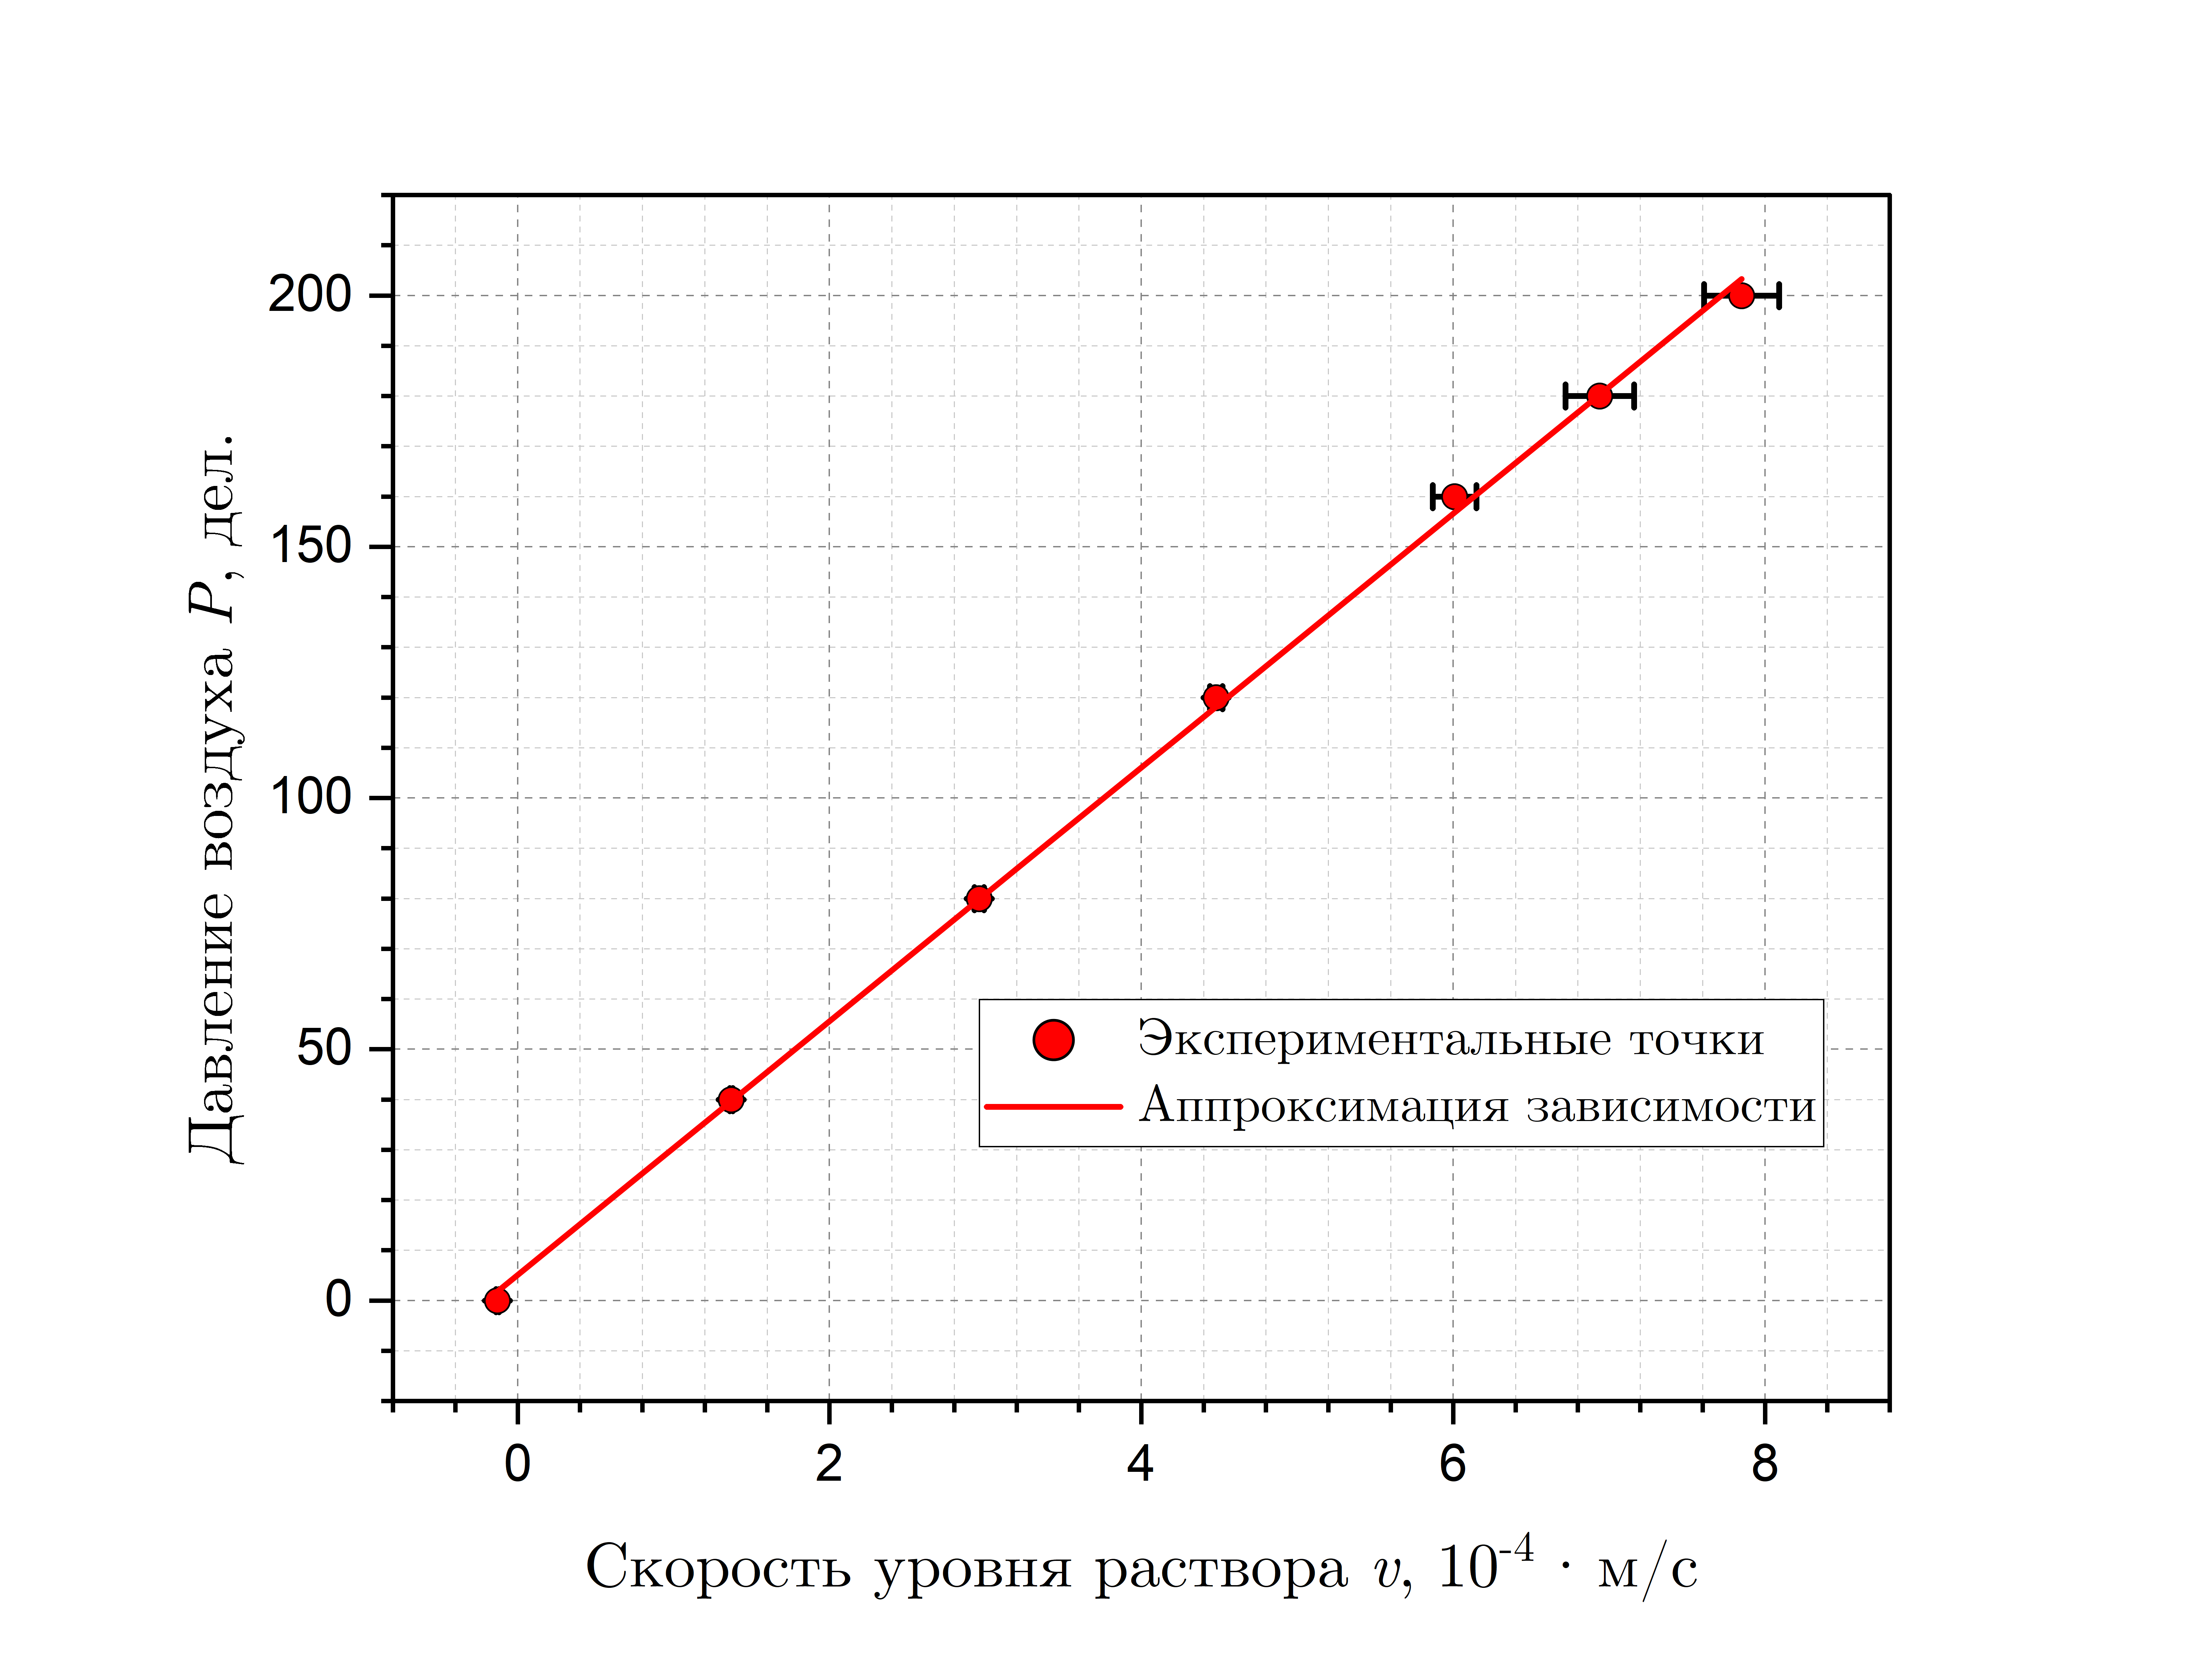
\includegraphics[width = 14 cm]{images/graph_15per.png}
            \caption{График зависимости $P(v)$ для второй концентрации раствора}
            \label{graph:15per}
        \end{figure}

        \subsection{Измерение осмотического давления для раствора концентрацией 0,075\%}
        
        \begin{table}[H]
            \centering
            \begin{tabular}{|c|ccccc|}
            \hline
            $P$, дел. & \multicolumn{1}{c|}{$t$, с} & \multicolumn{1}{c|}{$l$, см} & \multicolumn{1}{c|}{$u$, $10^{-4} \cdot$м/с} & \multicolumn{1}{c|}{$\overline{u}$, $10^{-4} \cdot$м/с} & $\sigma_{\overline{u}}$, $10^{-4} \cdot$м/с \\ \hline
            \multirow{5}{*}{200} & \multicolumn{1}{c|}{26,29} & \multicolumn{1}{c|}{\multirow{5}{*}{2}} & \multicolumn{1}{c|}{7,61} & \multicolumn{1}{c|}{\multirow{5}{*}{7,70}} & \multirow{5}{*}{0,12} \\ \cline{2-2} \cline{4-4}
             & \multicolumn{1}{c|}{25,51} & \multicolumn{1}{c|}{} & \multicolumn{1}{c|}{7,84} & \multicolumn{1}{c|}{} &  \\ \cline{2-2} \cline{4-4}
             & \multicolumn{1}{c|}{25,92} & \multicolumn{1}{c|}{} & \multicolumn{1}{c|}{7,72} & \multicolumn{1}{c|}{} &  \\ \cline{2-2} \cline{4-4}
             & \multicolumn{1}{c|}{25,52} & \multicolumn{1}{c|}{} & \multicolumn{1}{c|}{7,84} & \multicolumn{1}{c|}{} &  \\ \cline{2-2} \cline{4-4}
             & \multicolumn{1}{c|}{26,66} & \multicolumn{1}{c|}{} & \multicolumn{1}{c|}{7,50} & \multicolumn{1}{c|}{} &  \\ \hline
            \multirow{5}{*}{180} & \multicolumn{1}{c|}{30,41} & \multicolumn{1}{c|}{\multirow{5}{*}{2}} & \multicolumn{1}{c|}{6,58} & \multicolumn{1}{c|}{\multirow{5}{*}{6,69}} & \multirow{5}{*}{0,15} \\ \cline{2-2} \cline{4-4}
             & \multicolumn{1}{c|}{28,87} & \multicolumn{1}{c|}{} & \multicolumn{1}{c|}{6,93} & \multicolumn{1}{c|}{} &  \\ \cline{2-2} \cline{4-4}
             & \multicolumn{1}{c|}{30,11} & \multicolumn{1}{c|}{} & \multicolumn{1}{c|}{6,64} & \multicolumn{1}{c|}{} &  \\ \cline{2-2} \cline{4-4}
             & \multicolumn{1}{c|}{29,22} & \multicolumn{1}{c|}{} & \multicolumn{1}{c|}{6,84} & \multicolumn{1}{c|}{} &  \\ \cline{2-2} \cline{4-4}
             & \multicolumn{1}{c|}{30,88} & \multicolumn{1}{c|}{} & \multicolumn{1}{c|}{6,48} & \multicolumn{1}{c|}{} &  \\ \hline
            \multirow{5}{*}{160} & \multicolumn{1}{c|}{34,16} & \multicolumn{1}{c|}{\multirow{5}{*}{2}} & \multicolumn{1}{c|}{5,85} & \multicolumn{1}{c|}{\multirow{5}{*}{6,00}} & \multirow{5}{*}{0,16} \\ \cline{2-2} \cline{4-4}
             & \multicolumn{1}{c|}{34,71} & \multicolumn{1}{c|}{} & \multicolumn{1}{c|}{5,76} & \multicolumn{1}{c|}{} &  \\ \cline{2-2} \cline{4-4}
             & \multicolumn{1}{c|}{31,98} & \multicolumn{1}{c|}{} & \multicolumn{1}{c|}{6,25} & \multicolumn{1}{c|}{} &  \\ \cline{2-2} \cline{4-4}
             & \multicolumn{1}{c|}{32,71} & \multicolumn{1}{c|}{} & \multicolumn{1}{c|}{6,11} & \multicolumn{1}{c|}{} &  \\ \cline{2-2} \cline{4-4}
             & \multicolumn{1}{c|}{33,16} & \multicolumn{1}{c|}{} & \multicolumn{1}{c|}{6,03} & \multicolumn{1}{c|}{} &  \\ \hline
            \multirow{5}{*}{120} & \multicolumn{1}{c|}{44,95} & \multicolumn{1}{c|}{\multirow{5}{*}{2}} & \multicolumn{1}{c|}{4,45} & \multicolumn{1}{c|}{\multirow{5}{*}{4,48}} & \multirow{5}{*}{0,08} \\ \cline{2-2} \cline{4-4}
             & \multicolumn{1}{c|}{44,16} & \multicolumn{1}{c|}{} & \multicolumn{1}{c|}{4,53} & \multicolumn{1}{c|}{} &  \\ \cline{2-2} \cline{4-4}
             & \multicolumn{1}{c|}{43,55} & \multicolumn{1}{c|}{} & \multicolumn{1}{c|}{4,59} & \multicolumn{1}{c|}{} &  \\ \cline{2-2} \cline{4-4}
             & \multicolumn{1}{c|}{44,23} & \multicolumn{1}{c|}{} & \multicolumn{1}{c|}{4,52} & \multicolumn{1}{c|}{} &  \\ \cline{2-2} \cline{4-4}
             & \multicolumn{1}{c|}{46,48} & \multicolumn{1}{c|}{} & \multicolumn{1}{c|}{4,30} & \multicolumn{1}{c|}{} &  \\ \hline
            \multirow{5}{*}{80} & \multicolumn{1}{c|}{33,66} & \multicolumn{1}{c|}{\multirow{5}{*}{1}} & \multicolumn{1}{c|}{2,97} & \multicolumn{1}{c|}{\multirow{5}{*}{2,97}} & \multirow{5}{*}{0,01} \\ \cline{2-2} \cline{4-4}
             & \multicolumn{1}{c|}{33,29} & \multicolumn{1}{c|}{} & \multicolumn{1}{c|}{3,00} & \multicolumn{1}{c|}{} &  \\ \cline{2-2} \cline{4-4}
             & \multicolumn{1}{c|}{33,63} & \multicolumn{1}{c|}{} & \multicolumn{1}{c|}{2,97} & \multicolumn{1}{c|}{} &  \\ \cline{2-2} \cline{4-4}
             & \multicolumn{1}{c|}{33,93} & \multicolumn{1}{c|}{} & \multicolumn{1}{c|}{2,95} & \multicolumn{1}{c|}{} &  \\ \cline{2-2} \cline{4-4}
             & \multicolumn{1}{c|}{33,69} & \multicolumn{1}{c|}{} & \multicolumn{1}{c|}{2,97} & \multicolumn{1}{c|}{} &  \\ \hline
            40 & \multicolumn{5}{c|}{столб медленно опускается} \\ \hline
            20 & \multicolumn{5}{c|}{столб медленно понижается} \\ \hline
            10 & \multicolumn{5}{c|}{столб медленно поднимается} \\ \hline
            \multirow{5}{*}{0} & \multicolumn{1}{c|}{56,32} & \multicolumn{1}{c|}{\multirow{5}{*}{0,1}} & \multicolumn{1}{c|}{0,18} & \multicolumn{1}{c|}{\multirow{5}{*}{0,18}} & \multirow{5}{*}{0,01} \\ \cline{2-2} \cline{4-4}
             & \multicolumn{1}{c|}{57,28} & \multicolumn{1}{c|}{} & \multicolumn{1}{c|}{0,17} & \multicolumn{1}{c|}{} &  \\ \cline{2-2} \cline{4-4}
             & \multicolumn{1}{c|}{56,69} & \multicolumn{1}{c|}{} & \multicolumn{1}{c|}{0,18} & \multicolumn{1}{c|}{} &  \\ \cline{2-2} \cline{4-4}
             & \multicolumn{1}{c|}{56,98} & \multicolumn{1}{c|}{} & \multicolumn{1}{c|}{0,18} & \multicolumn{1}{c|}{} &  \\ \cline{2-2} \cline{4-4}
             & \multicolumn{1}{c|}{57,91} & \multicolumn{1}{c|}{} & \multicolumn{1}{c|}{0,17} & \multicolumn{1}{c|}{} &  \\ \hline
            \end{tabular}
            \caption{Результаты измерений для третьей концентрации раствора}
            \label{table:0.75per}
        \end{table}

        \noindent Построим график зависимости (рис. \ref{graph:75per}) давления воздуха $P$ от изменения скорости $v$ движения уровня раствора в капилляре для раствора с концентрацией $0,075 \%$. \\

        \noindent Аппроксимацию прямой произведем методом наименьших квадратов в компьютерной программе \textit{Origin Pro 2023}, в которой определим координату пересечения графика $P(v)$ с осью ординат. Получим:

        $$
        \boxed{P_\text{осм} = 4,6 \pm 1,8 \text{ дел} = 1127 \pm 441 \text{ Па}}
        $$

        \begin{figure}[H]
            \centering
            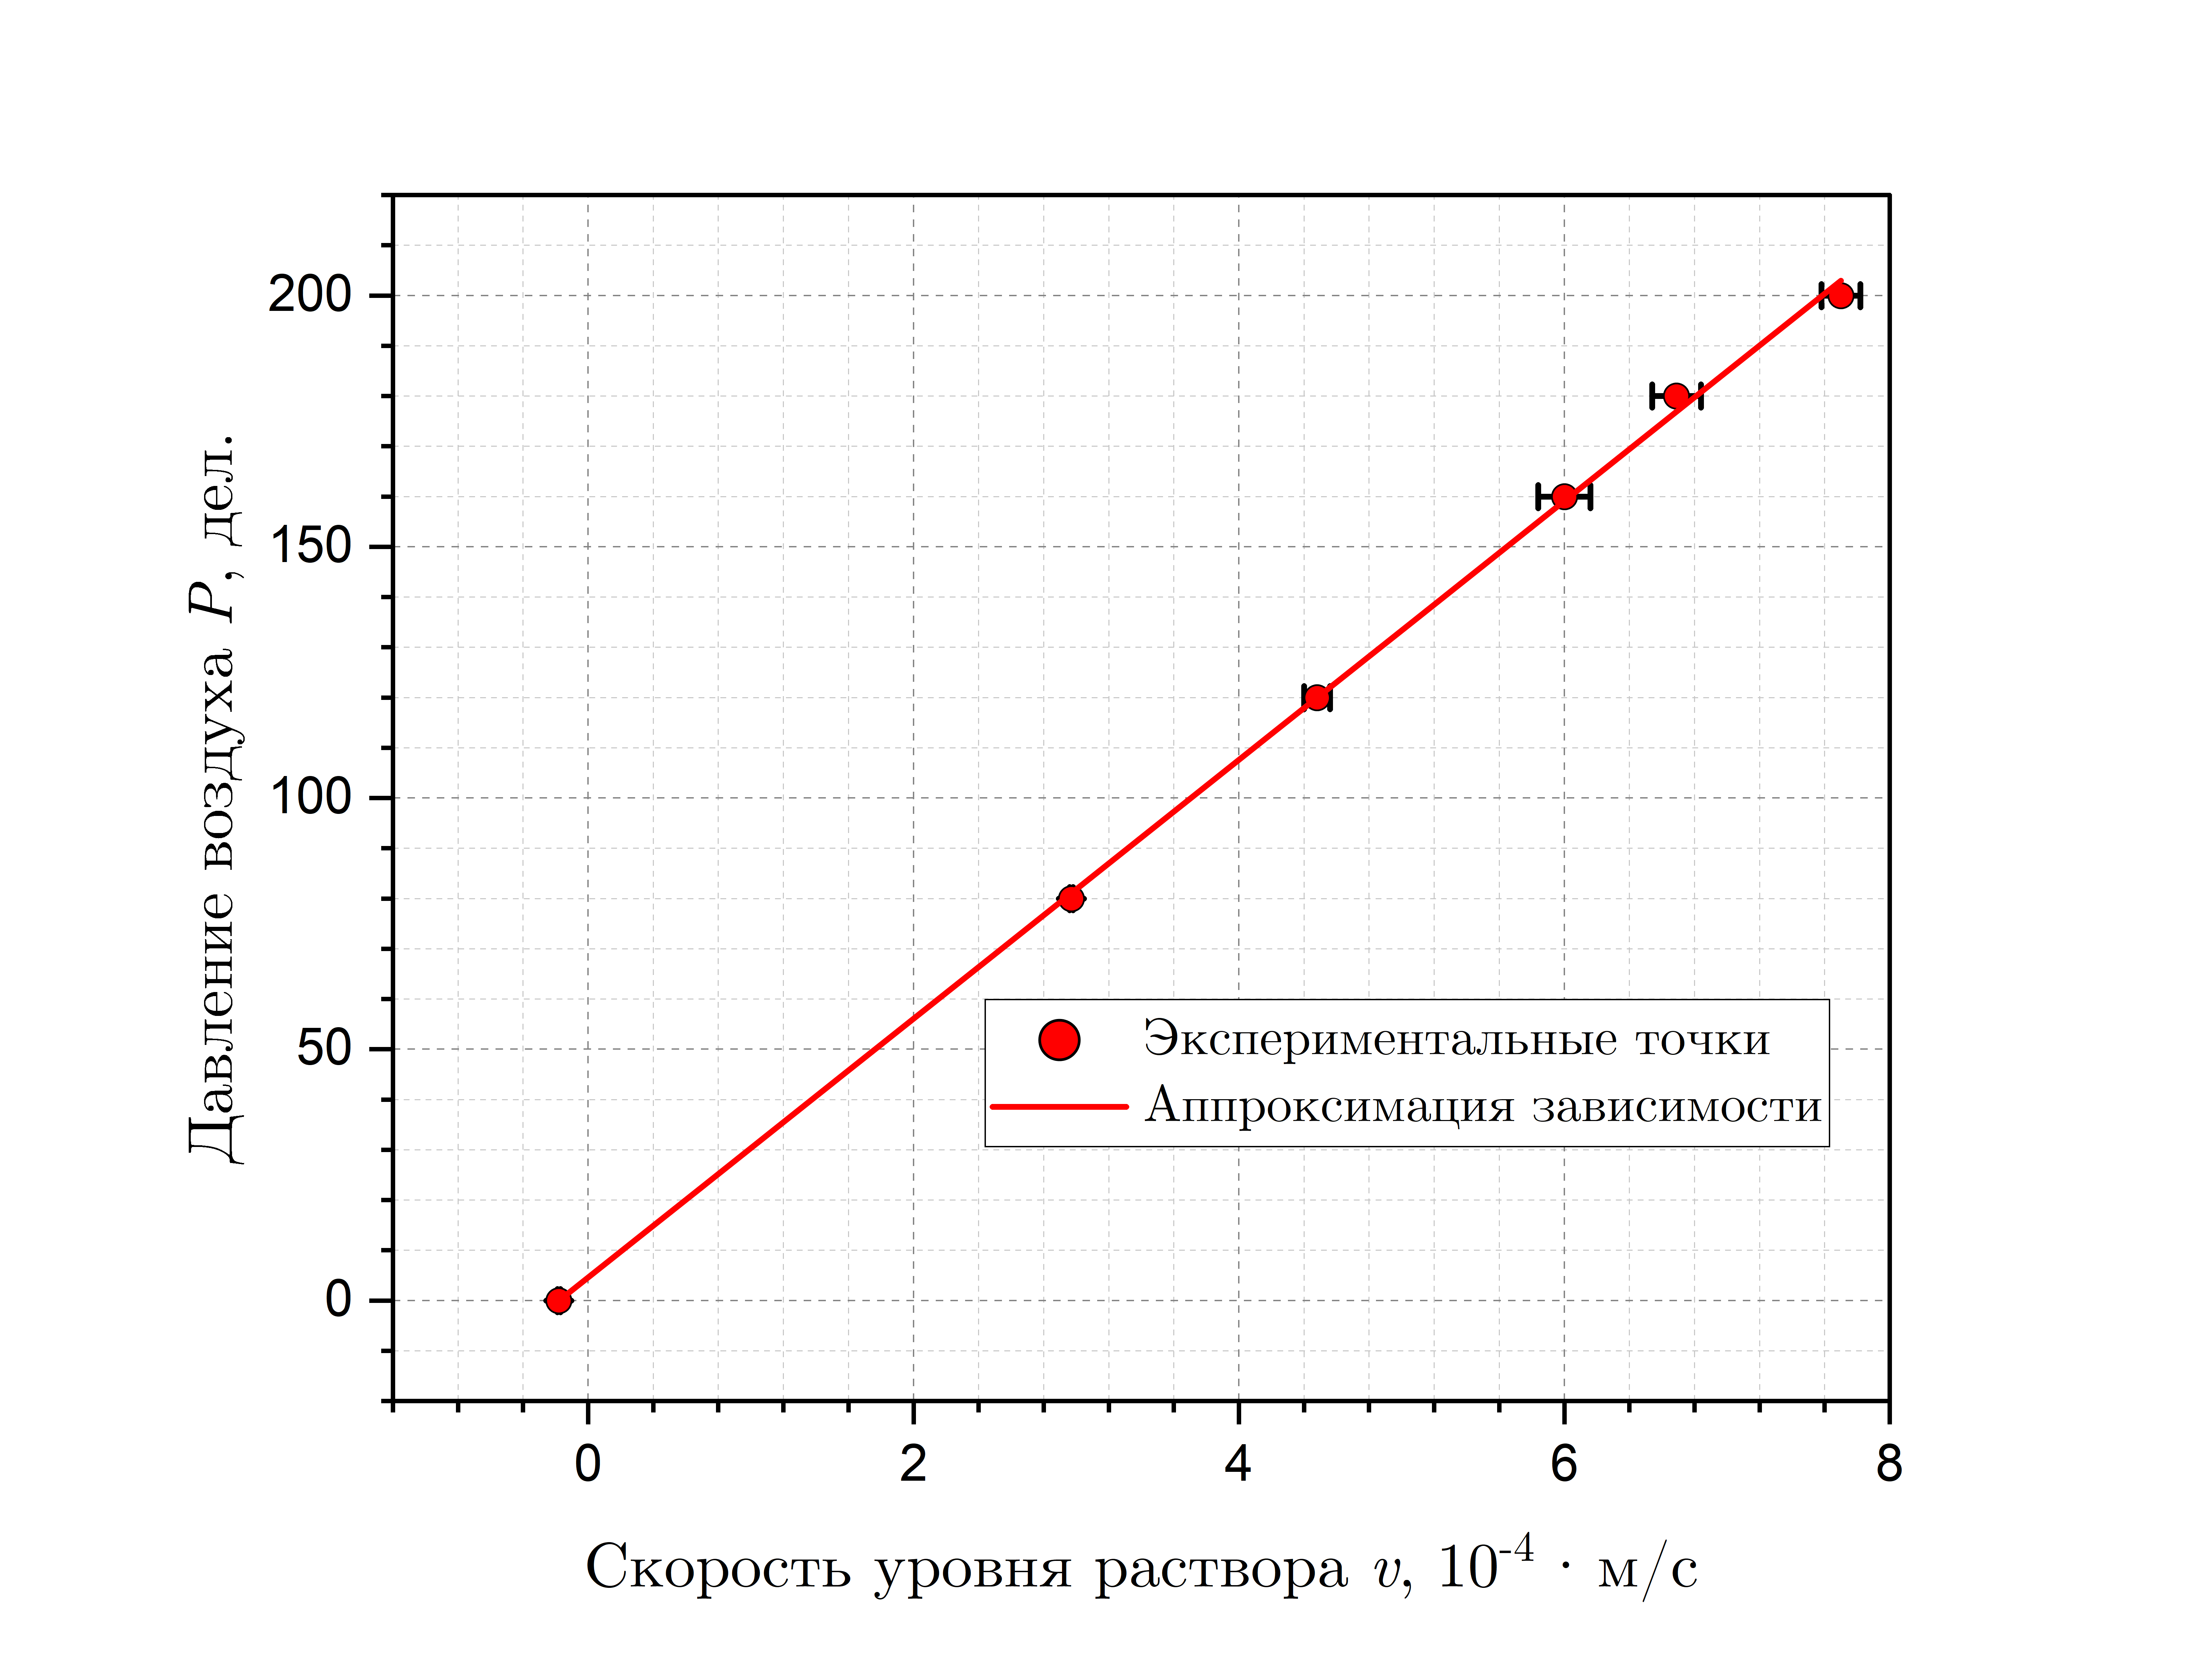
\includegraphics[width = 14 cm]{images/graph_75per.png}
            \caption{График зависимости $P(v)$ для третьей концентрации раствора}
            \label{graph:75per}
        \end{figure}

    \newpage

    \subsection{Измерение зависимости осмотического давления от концентрации раствора}

    \noindent По результатам предыдущих пунктов заполним таблицу \ref{table:osm}. По данной таблице построим график зависимости (рис. \ref{graph:osm}) осмотического давления $P_\text{осм}$ от концентрации раствора $n$. Аппроксимацию прямой произведем методом наименьших квадратов в компьютерной программе \textit{Origin Pro 2023}.

    \begin{table}[H]
        \centering
        \begin{tabular}{|c|c|c|c|c|c|}
        \hline
        $n, \%$ & $P_\text{осм}$, дел. & $\sigma_{P_\text{осм}}$, дел. & $P_\text{осм}$, Па & $\sigma_{P_\text{осм}}$, Па & $P_\text{В.--Г.}$, Па \\ \hline
        0,300 & 6,0 & 2,3 & 1470 & 564 & 19998 \\ \hline
        0,150 & 5,1 & 1,6 & 1250 & 392 & 9999 \\ \hline
        0,075 & 4,6 & 1,8 & 1127 & 441 & 5000 \\ \hline
        \end{tabular}
        \caption{Зависимость осмотического давления от концентрации}
        \label{table:osm}
    \end{table}

    \begin{figure}[H]
        \centering
        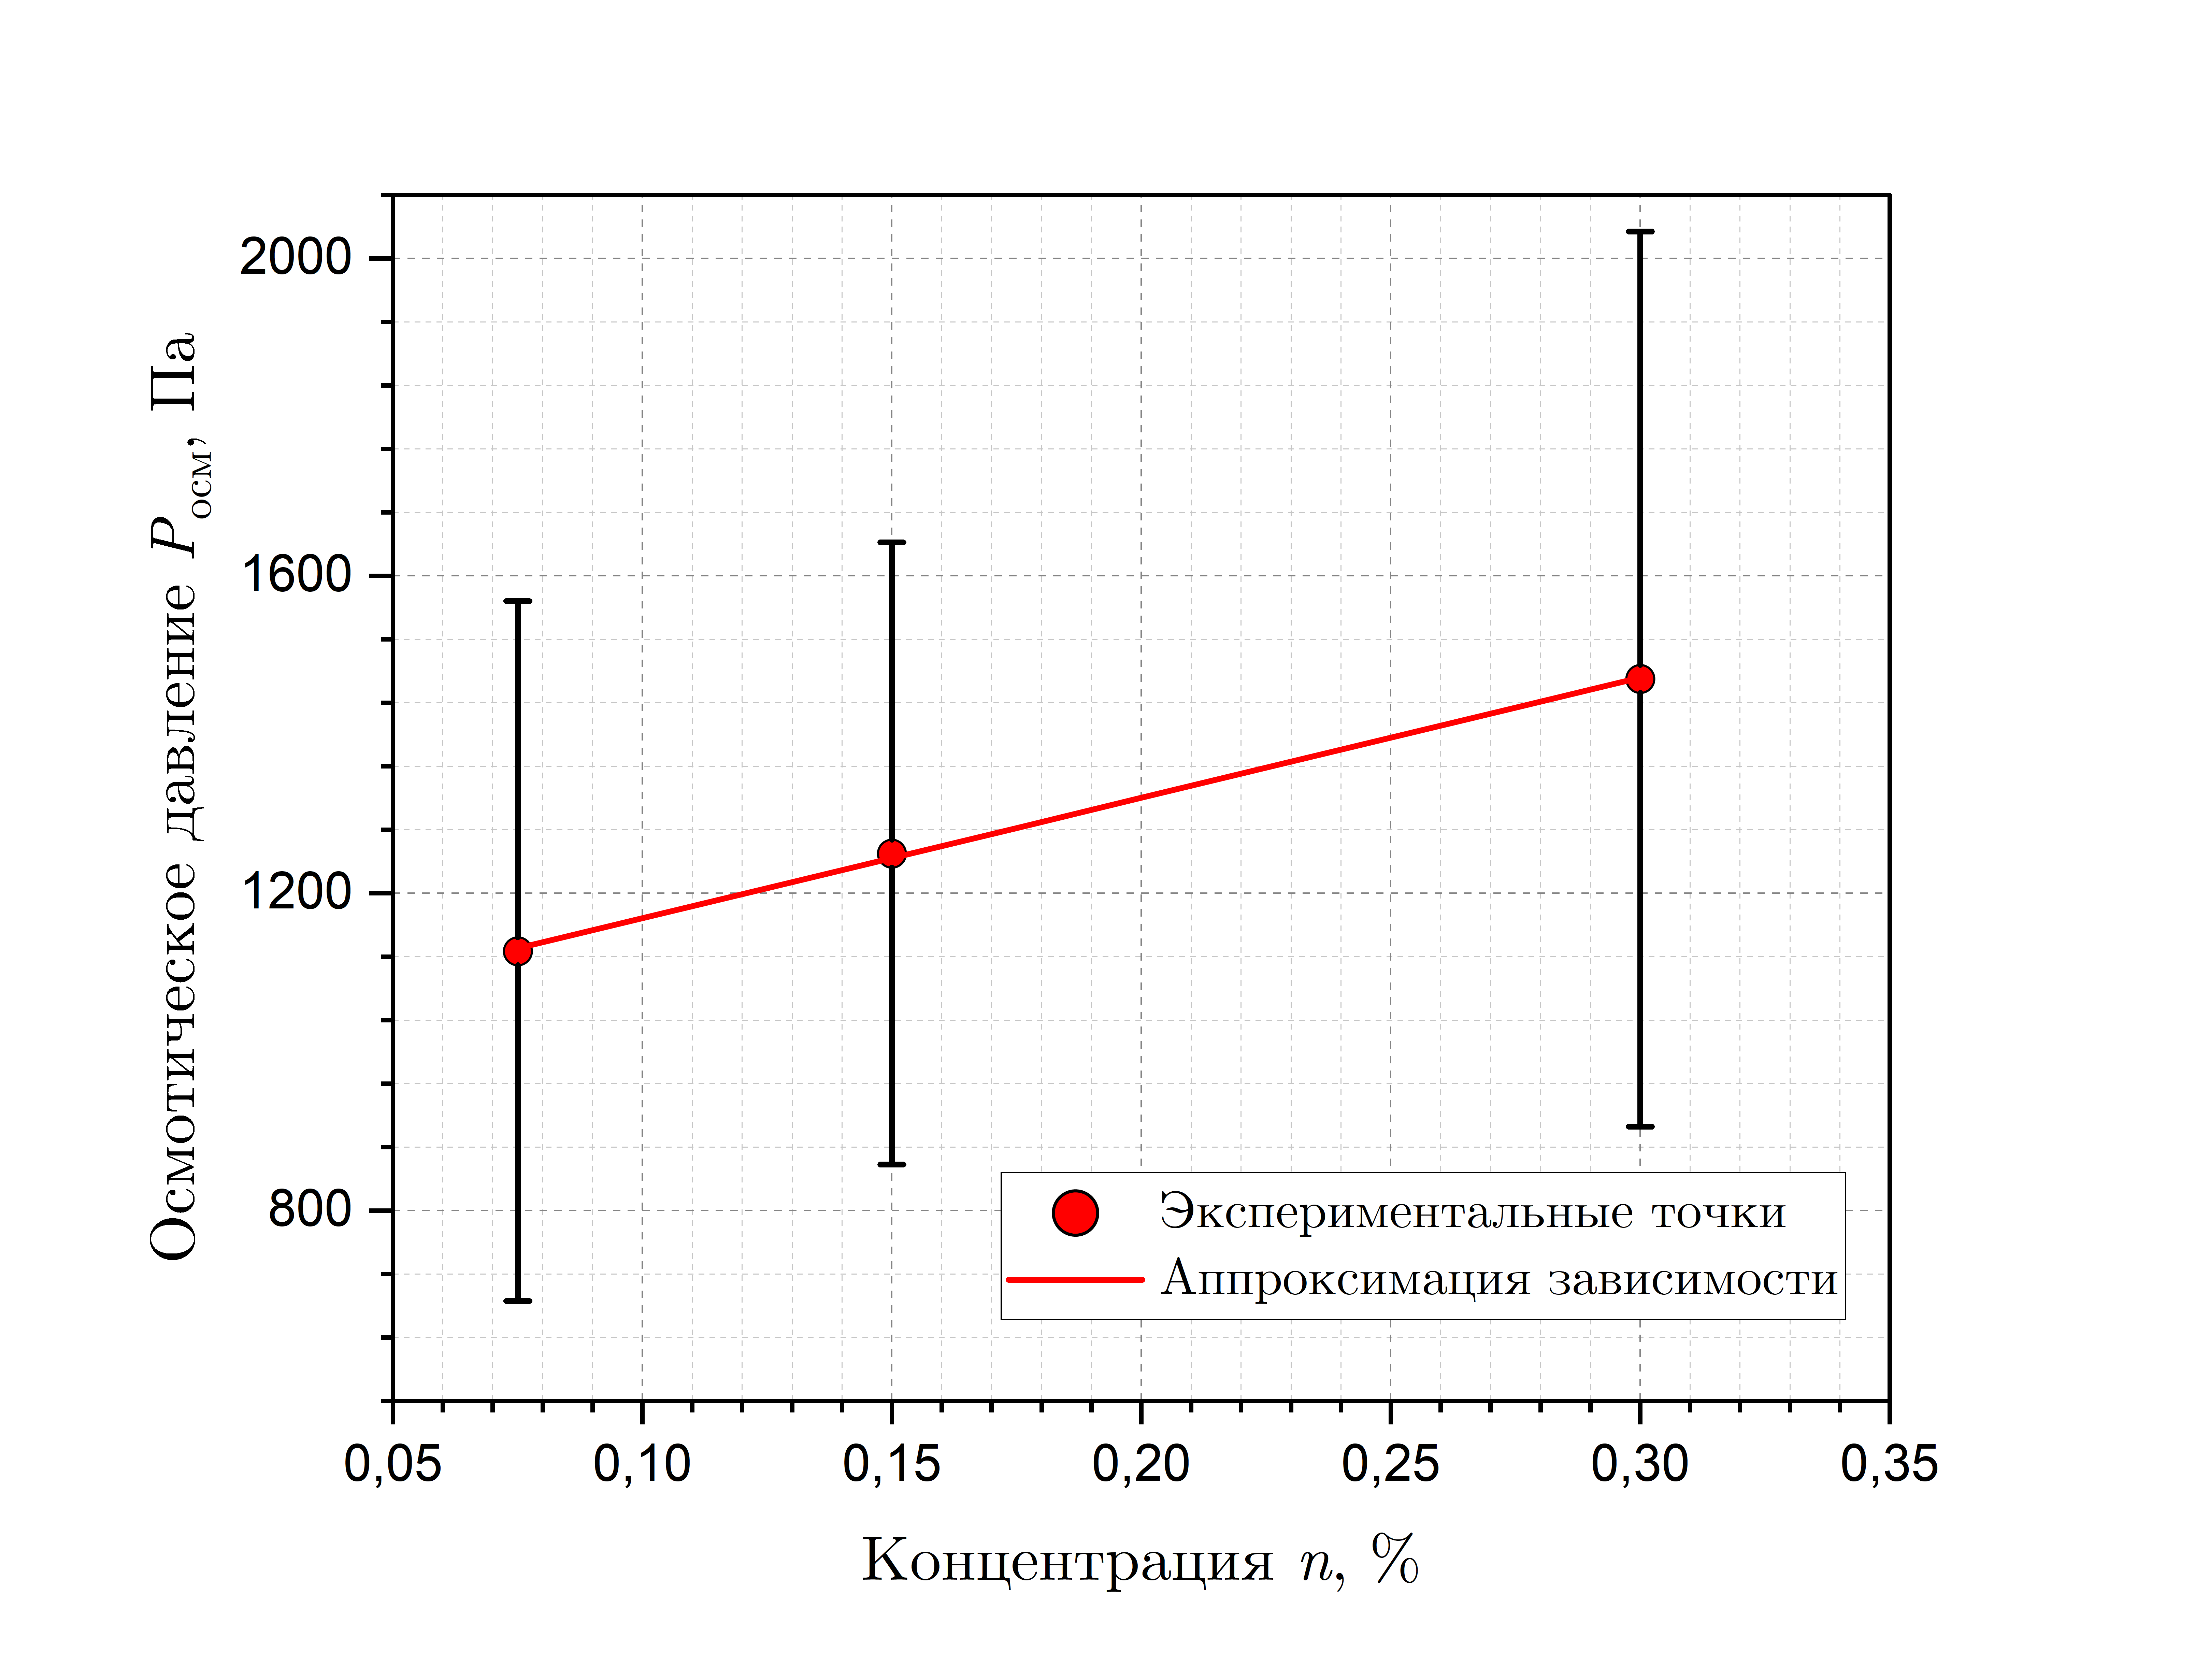
\includegraphics[width = 14 cm]{images/graph_osm.png}
        \caption{График зависимости $P_\text{осм}(n)$}
        \label{graph:osm}
    \end{figure}

    \noindent Теперь сравним полученные экспериментальные данные с теоретическими, для этого преобразуем закон Вант-Гоффа:
    $$
        P_\text{В.--Г.} = nkT = \frac{N_\text{соли} \cdot k T}{V_\text{воды}} = \frac{N_\text{соли} \cdot k T \cdot \rho_\text{воды}}{M_\text{воды}} = \frac{N_A \nu_\text{соли} \cdot k T \cdot \rho_\text{воды}}{М_\text{воды}}
    $$

    \noindent Отсюда, получим:

    \begin{equation}
        \label{eq:osm_vg}
        P_\text{В.--Г.} = \frac{RT \cdot m_\text{соли} \cdot \rho_\text{воды}}{M_\text{воды} \cdot \mu_\text{соли}} = \frac{RT \cdot \rho_\text{воды} \cdot n[\%]}{\mu_\text{соли} \cdot 100 \%}
    \end{equation}

    \noindent По формуле \ref{eq:osm_vg} вычислим значения осмотических давлений $P_\text{В.--Г.}$ для трёх разных концентраций, указанных в таблице \ref{table:osm} и занесём в неё полученные результаты. \\

    \noindent Построим график зависимости (рис. \ref{graph:unity}) осмотического давления $P_\text{В.--Г.}$ от концентрации $n$ по \textit{закону Вант-Гоффа}.

     \begin{figure}[H]
        \centering
        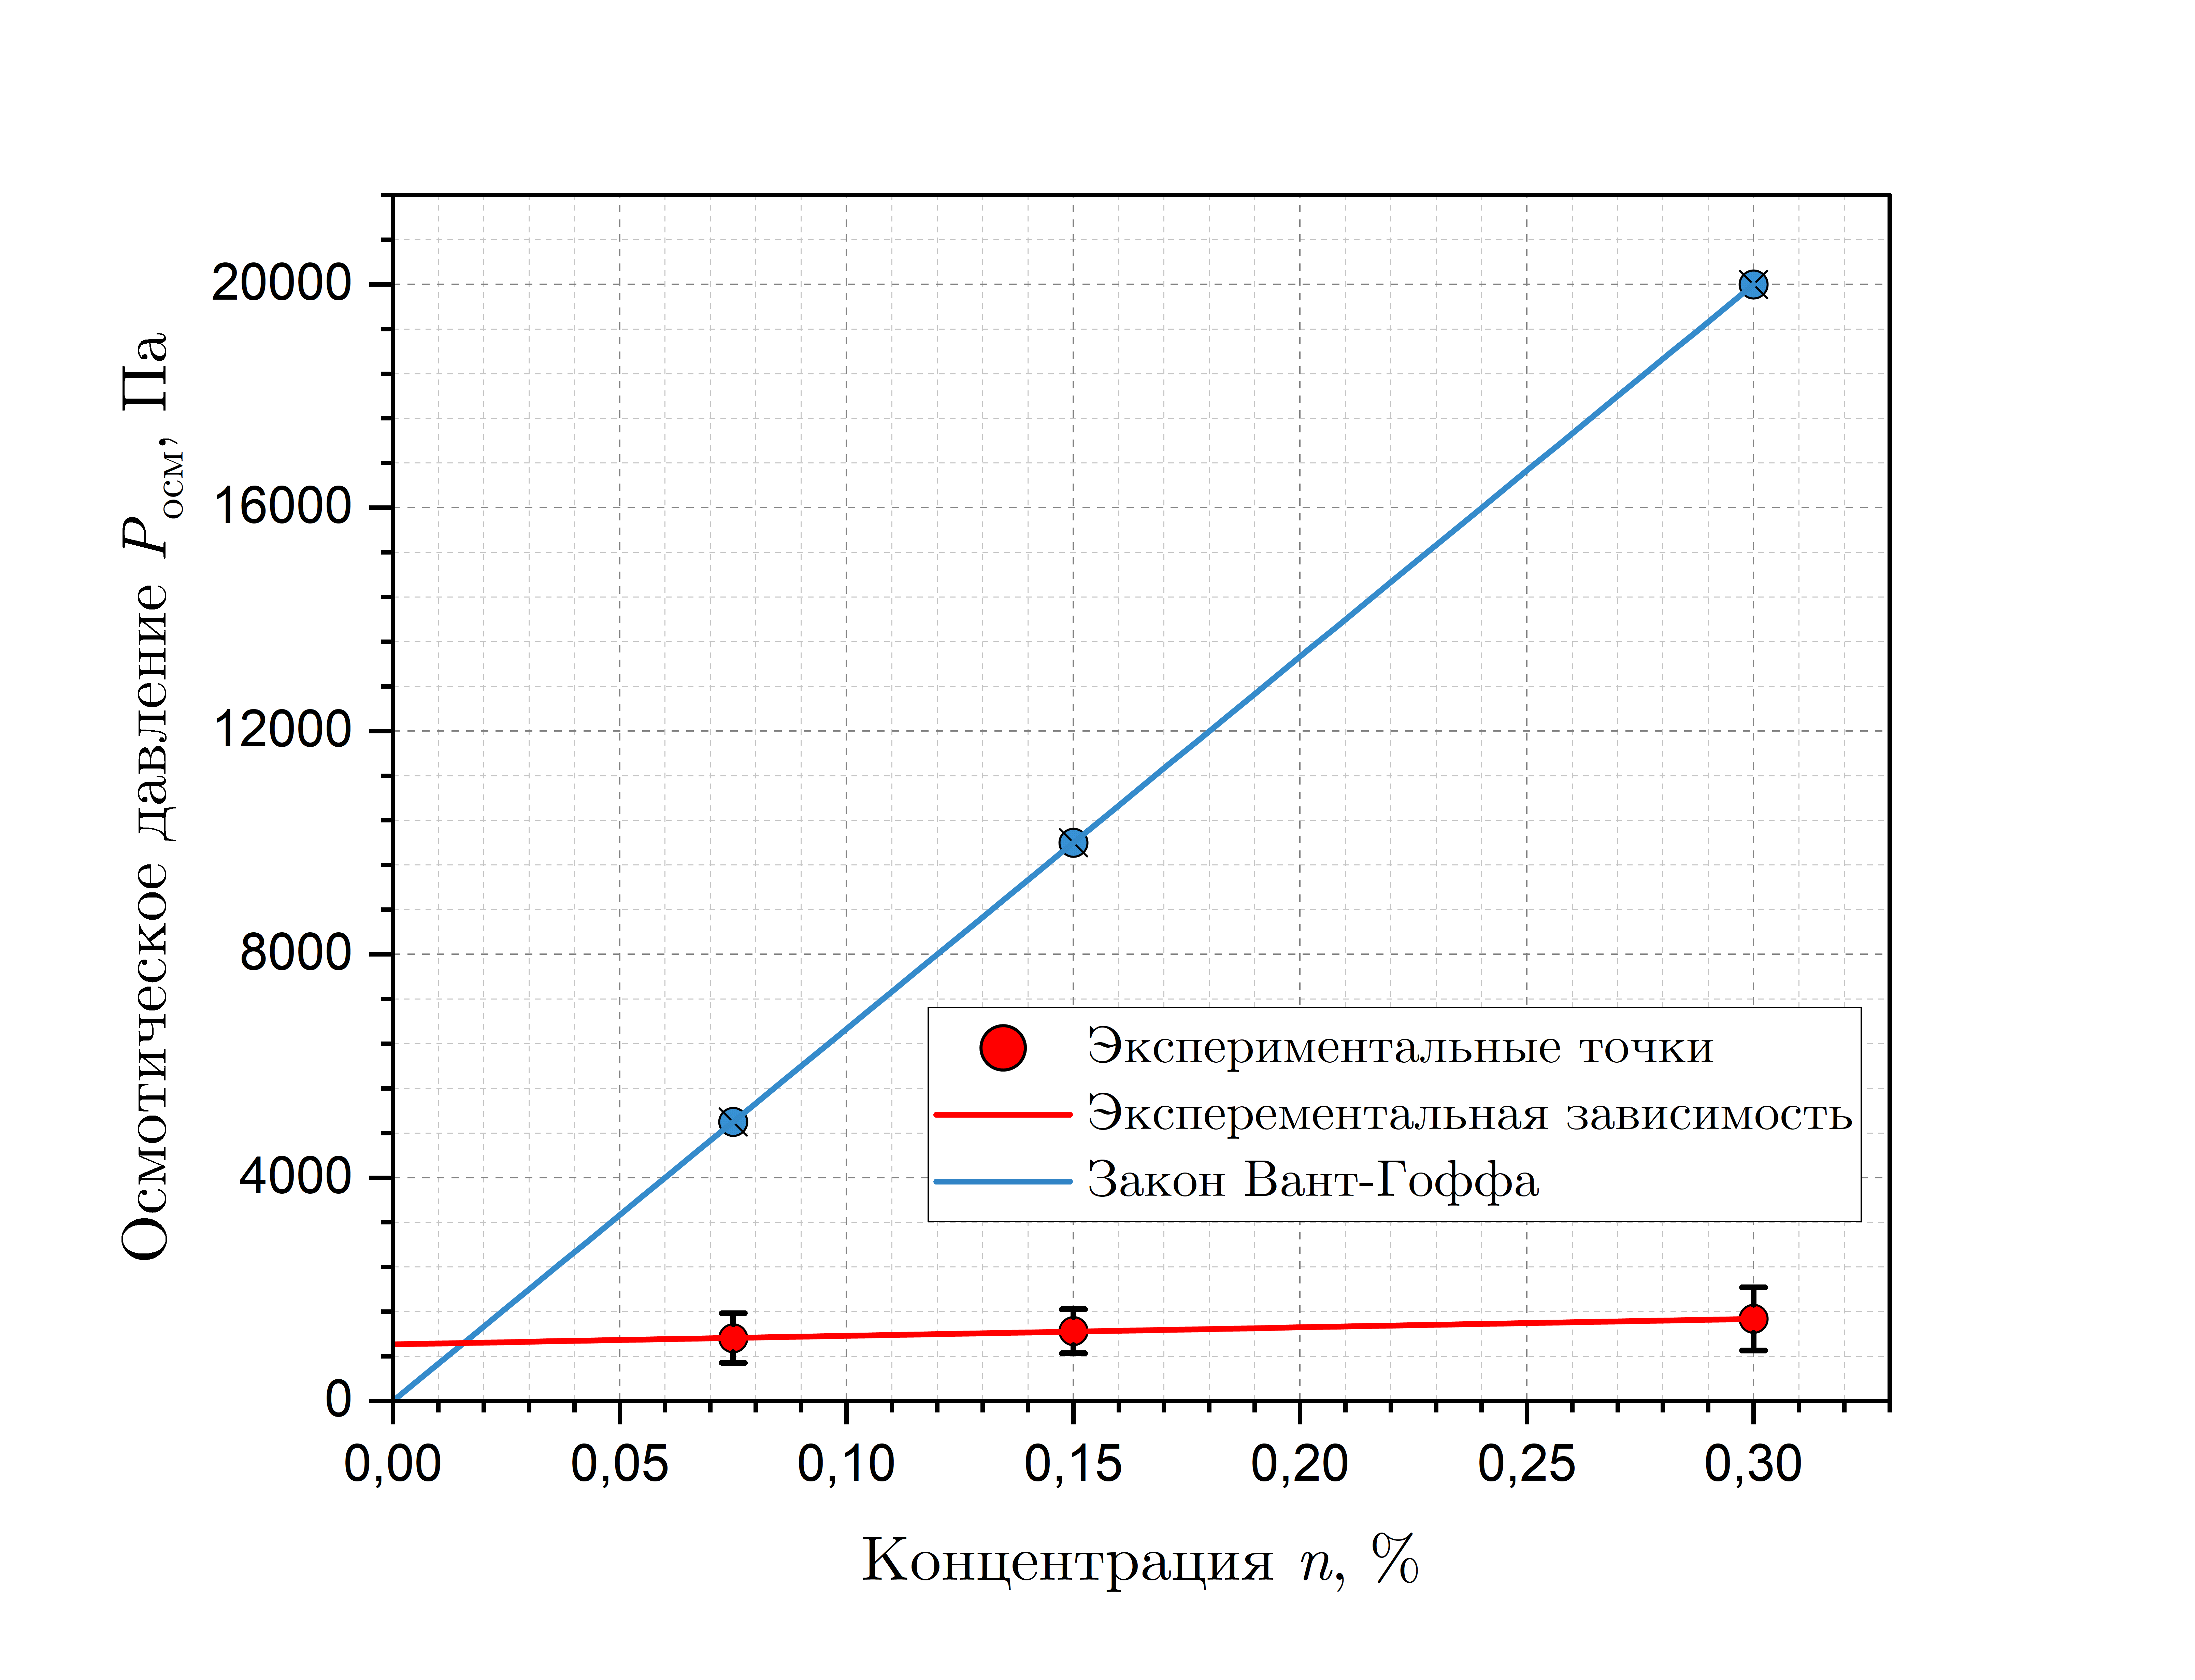
\includegraphics[width = 14 cm]{images/graph_unity.png}
        \caption{Объединённый график зависимости $P_\text{осм}(n)$}
        \label{graph:unity}
    \end{figure}
    
    \section{Заключение}
    
    \noindent В работе наблюдался прямой и обратный осмос, было измерено осмотическое давление при разной концентрации раствора. Проверить закон Вант-Гоффа не удалось, измеренное осмотическое давление не совпадает с вычисленным. Сложно определить, является ли зависимость $P_{осм}$ линейной, так как для этого нужно проводить измерения при большем числе концентраций. \\

    \noindent На результат эксперимента могли повлиять следующие факторы:
    \begin{itemize}
        \item во время измерений было обнаружено падение давления в системе на $\approx 3$ деления манометра. Течь устранить не удалось. Негерметичность системы могла повлиять на итоговые значения;
        \item ошибки в приготовлении и разбавлении раствора;
        \item полупроницаемые перегородки давно не менялись и со временем могли засориться, что приводит к уменьшению скорости протекания осмоса и понижению измеренного давления от вычисленного по формуле Вант-Гоффа, из-за этого точки при $P = 0 \text{ дел.}$ на графиках \ref{graph:3per}, \ref{graph:15per} и \ref{graph:75per} отклоняются от прямой.
    \end{itemize}

\end{document}